%--------------------------------- Framework -------------------------------------------------------
\subsection{Proposed Framework considering V\textsubscript{th} Assignment}
\label{sec:TVA:framework}
\begin{figure}
	\centering
	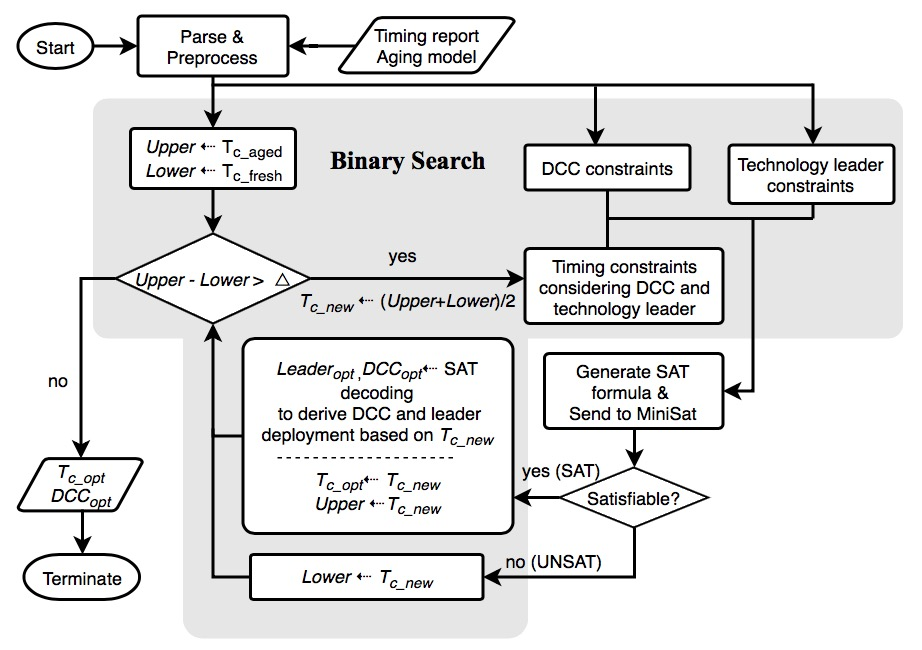
\includegraphics[width=0.9\columnwidth]{Flow_chart_tva.png}
	\caption{The overall flow of the framework when technology leaders are considered }
	\label{fig:flow:tva}
\end{figure}
The proposed framework, which simultaneously considers aging manipulation (DCC) and V\textsubscript{th} assignment (technology leader), is depicted in Figure~\ref{fig:flow:tva}. Compared with the former framework in Figure~\ref{fig:flow}, the framework is also based on a binary search for the minimum clock period ($T_c$) and SAT formulation, while timing constraints need to consider the technology leader selection. The problem, technology leader selection from clock buffers, is formulated as SAT problem, and so is the problem of DCC insertion/deployment. In the sequel, Section~\ref{sec:TVA:leader_encode} explains how the problem of DCC insertion and technology leader selection is encoded by Boolean variables. Section~\ref{sec:TVA:constraints} reviews DCC constraints and introduces technology leader constriants. Section~\ref{sec:TVA:timingconstraint} introduces the timing constraints which consider DCC deployment and technology leader selection.

%--------------------------------- Encoding -------------------------------------------------------
% (5)
\subsubsection{Encoding for DCC and Technology Leader Deployment}
\label{sec:TVA:leader_encode}
The problem of DCC deployment and technology leader selection needs to be encoded into Boolean representation before being transformed into a SAT-based formulation. Assume that a total of $N$ types of DCCs can be chosen. Including the DCC-free case where no DCC is inserted, there are ($N$ + 1) possibilities of DCC insertion for each clock buffer. Furthermore, we also assume that a total of $M$ types of technology leaders can be chosen. Note that, each type of technology leader represents an individual technology. Including the nominal technology, there are ($M$ + 1) possibilities of technology leader selection for each clock buffer. We denote a clock buffer by $p\left(1 \leq p \leq P\right)$ where $P$ is the total count of clock buffers and $p$ is buffer index. For each clock buffer, there exist two types of Boolean variables, $B_{p,q}$ and $B_{p,r}$ ($1 \leq q \leq Q < r \leq R$, $Q = \lceil \lg (N + 1)\rceil$ and $R = \lceil \lg \{(N + 1)(M + 1\}\rceil$), where $\left\{B_{p,1}, B_{p,2},\dotsc, B_{p,Q}\right\}$ encode the aforementioned ($N$ + 1) possibilities of DCC insertion at the input of buffer $p$ and $\left\{B_{p,Q+1}, B_{p,Q+2},\dotsc, B_{p,R}\right\}$ encode the ($M$ + 1) possibilities of leader selection of buffer $p$.
%The problem of DCC deployment and technology leader selection needs to be encoded into Boolean representation before being transformed into a SAT-based formulation. Assume that a total of $N$ types of DCCs can be chosen. Including the DCC-free case where no DCC is inserted, there are ($N$ + 1) possibilities of DCC insertion for each clock buffer. Furthermore, we also assume that a total of $M$ types of technology leaders can be chosen. Note that, each type of technology leader represents an individual technology. Including the nominal technology, there are ($M$ + 1) possibilities of technology leader selection for each clock buffer. We denote a clock buffer by $p\left(1 \leq p \leq P\right)$ where $P$ is the total count of clock buffers. For each clock buffer, there exist two types of Boolean variables, $B_{p,q}$ and $B_{p,r}$, where $1 \leq p \leq P$, $1 \leq q \leq Q \leq r \leq R$, $Q = \lceil \lg (N + 1)\rceil$ and $R = \lceil \lg \{(N + 1)(M + 1\}\rceil$. $B_{p,q}$ are used to encode the ($N$ + 1) possibilities of DCC insertion, and $B_{p,r}$ are used to encode the ($M$ + 1) possibilities of technology leader selection.


\begin{figure}
    \centering
    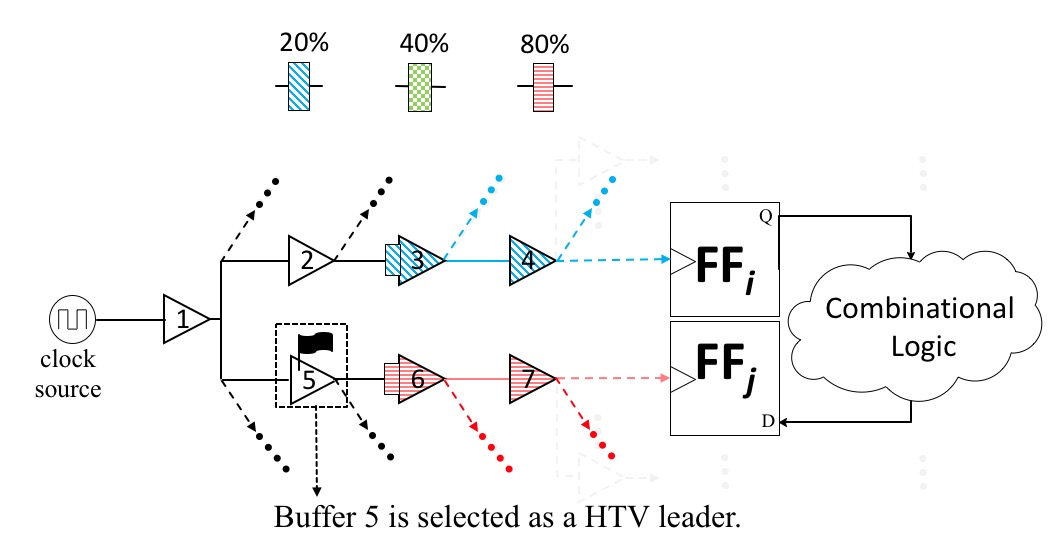
\includegraphics[width=0.9\columnwidth]{example_of_dcc_leader.png}
    \caption{An example with DCC deployment and technology selection}
    \label{fig:example_dcc_tva}
\end{figure}

Without loss of generality, we assume $N$ = 3, and $M$ = 1. Thus, there are three types of DCCs, which are assumed to be 20\%, 40\%, and 80\% DCCs, as shown in Figure~\ref{fig:dcctype}. In addition, there is one type of technology leader, which is assumed to be high-V\textsubscript{th} leader. Note that, if the clock buffer is selected as the high-V\textsubscript{th} leader, the technology of the buffer and the associated downstream ones is replaced with high-V\textsubscript{th} counterpart. Since we assume three types of DCC and one type of technology leader, three Boolean variables are used for encoding eight possibilities of DCC and technology leader at any buffer. The eight possibilities can be encoded as follows:

{\small
\begin{tabular}{  c  c  c  c  }
  	 & Leader type & DCC type & $\{B_{p,3}, B_{p,2}, B_{p,1}\}$ \\ 
  	(1)\quad & Nominal V\textsubscript{th} & None & \{0, 0, 0\} \\ 
  	(2)\quad & Nominal V\textsubscript{th} &20\% &  \{0, 0, 1\} \\ 
  	(3)\quad & Nominal V\textsubscript{th} &40\% &  \{0, 1, 0\} \\ 
  	(4)\quad & Nominal V\textsubscript{th} &80\% &  \{0, 1, 1\} \\ 
	(5)\quad & high-V\textsubscript{th} & None & \{1, 0, 0\} \\ 
  	(6)\quad & high-V\textsubscript{th} & 20\% &  \{1, 0, 1\} \\ 
  	(7)\quad & high-V\textsubscript{th} & 40\% &  \{1, 1, 0\} \\ 
  	(8)\quad & high-V\textsubscript{th} & 80\% &  \{1, 1, 1\} \\ 
\end{tabular}}


For example, in Figure~\ref{fig:example_dcc_tva}, the DCC deployment is same with that in Figure~\ref{fig:sub:dcci2} (i.e., 20\% DCC at buffer 3 and 80\% DCC at buffer 6), but the buffer 5 is selected as the high-V\textsubscript{th} leader, which is denoted by a black flag. Thus, the technology of buffer 5, 6 and 7 is replaced with the high-V\textsubscript{th} counterpart. Therefore, {\small $\left\{B_{3,3}, B_{3,2}, B_{3,1}\right\}$ = \{0, 0, 1\}}, {\small $\left\{B_{5,3}, B_{5,2}, B_{5,1}\right\}$ = \{1, 0, 0\}}, {\small $\left\{B_{6,3}, B_{6,2}, B_{6,1}\right\}$ = \{0, 1, 1\}}, and {\small $\left\{B_{p,3}, B_{p,2}, B_{p,1}\right\}$ = \{0, 0, 0\}} for $p$ = 1, 2, 4 or 7.

As mentioned in Section~\ref{subsec:eddcd}, the 20\% DCC mitigates the aging of buffer 3 and its downstream buffers, but the 80\% DCC aggravates the aging of buffer 6 and its downstream buffers. Moreover, since the buffer 5 is a high-V\textsubscript{th} leader, buffer 5, 6 and 7 are changed as high-V\textsubscript{th} buffers, implying the latency from buffer 5 to buffer 7 is lengthened. This way, the clock skew becomes larger than that in Figure~\ref{fig:sub:dcci2}, so that the required $T_c$ can be further reduced, based on time borrowing. Note that, as we mentioned in Section~\ref{sec:TVA:example}, the $T_c$ reduction in Figure~\ref{fig:sub:dcci2} is only due to the useful aging-induced clock skew; however, the  further $T_c$ reduction in Figure~\ref{fig:example_dcc_tva} is both based on useful aging-induced and tech-induced clock skew, which is caused by the V\textsubscript{th} assignment of clock buffers. 